\documentclass{article}
\usepackage[T1]{fontenc}
\usepackage{lmodern}
\usepackage{graphicx}
\usepackage{amsmath,amssymb}
\usepackage[a4paper,margin=2cm]{geometry}
\usepackage[absolute,overlay]{textpos}
\setlength{\TPHorizModule}{1mm}
\setlength{\TPVertModule}{1mm}
\usepackage[indonesian]{babel}
\usepackage{hyperref}
\setlength{\emergencystretch}{2em}
% unit: Halaman 99

\begin{document}

% === Halaman 99 (llm) ===

\begin{itemize}
  \item Cara menghitung matriks invers $2 \times 2$:
\end{itemize}

\vspace{20mm}

Contoh: $K = \begin{pmatrix} 3 & 10 \\ 15 & 9 \end{pmatrix}$

\[ \det(K) = (3)(9) - (15)(10) = 27 - 150 = -123 \pmod{26} = 7 \]

% deskripsi: Rumus umum invers matriks 2x2
% bbox normalisasi: [0.1100, 0.2070, 0.6480, 0.5530]
\begin{textblock*}{112.98mm}(23.10mm,61.48mm)
\noindent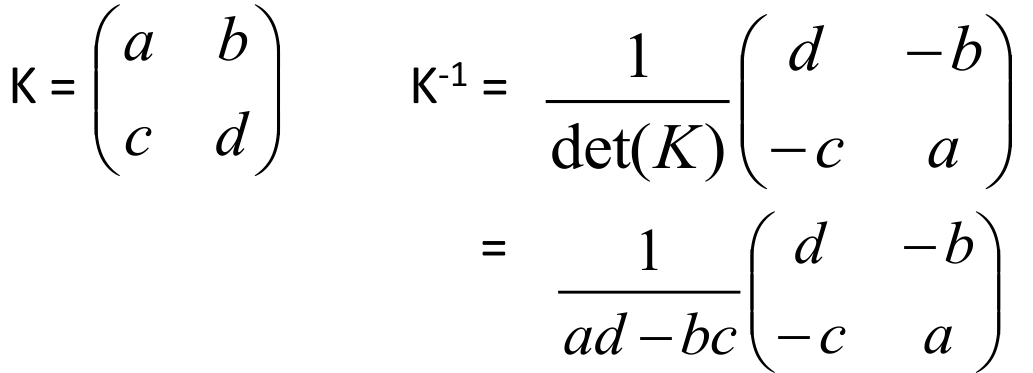
\includegraphics[width=112.98mm,height=102.76mm]{../../images/llm/page_099_img_01.png}%
\end{textblock*}

\end{document}
